%% =====================================================================
%%  5_results.tex  Chapter 5: Results and Discussion
%%  v18. Merge of author base (current-static-checks kept) with prior-round
%%  edits: over-rejection reword, placebo + ablation-null justification,
%%  auxiliary-operations defence, supplier sentence removed (figure to
%%  threats), PI supplier column dropped, numbers in numeral form.
%% =====================================================================

\chapter{Results and Discussion} \label{chap:results}

This chapter evaluates the artefact designed in Chapter~\ref{chap:method} against the empirical material prepared in Chapter~\ref{chap:empirical}. Section~\ref{sec:results:comparison} compares the 5 pipeline designs on document level disposition, paired contrasts, per rule behaviour, cost and latency, and the supplier context ablation. Section~\ref{sec:results:position} isolates the effect of the position of the deterministic enforcer, and Section~\ref{sec:results:errors} analyses the errors. The findings are answered against the research questions, and the limitations consolidated, in Chapter~\ref{chap:conclusions}.


%% =================================================================
\section{Introduction}
\label{sec:results:intro}

The evaluation compares 5 pipeline designs: the pure LLM design, the post hoc design, the LLM-as-judge design, the in generation design, and the pre hoc design. The post hoc, in generation and pre hoc designs each embed a deterministic enforcer at a different point of the pipeline; the pure LLM and LLM-as-judge designs do not. The contrast between these 2 groups answers the first part of the analysis, and the contrast among the 3 enforcer positions answers the second.

The reporting is structured by 3 research questions. RQ.1 asks how the 5 designs compare on per rule accuracy, document level disposition, cost and latency. RQ.2 asks whether the position of the deterministic enforcer affects accuracy, cost and latency. RQ.3 asks whether conditioning the prompt on a supplier's historical failure record improves accuracy. Section~\ref{sec:results:comparison} addresses RQ.1, Section~\ref{sec:results:position} addresses RQ.2, and Section~\ref{sec:results:rag} addresses RQ.3.

Three rule counts recur and are kept distinct throughout. The register has 22 rules. Per rule recall is reported over the 20 evaluable rules, excluding R11 (a schema entry check that fires before rule evaluation) and R18 (a stateful duplicate rule tested by a separate re-submission check); on each cohort it is measured at the instance level, over the 41 single rule mutant targets on the synthetic sample and the 106 flagged rule cells on the buyer sample. A single static mutant exercises these rules one at a time, except R18, which needs re-submission, and R11 and R22, which carry N/A on every mutant for the reasons given in Section~\ref{sec:emp:synthetic}.

Two reporting conventions apply throughout. Every metric is the consensus across 5 repeated runs of the pipeline on each sample, so each case carries the majority verdict of its 5 runs, and the 5 designs appear in a fixed order, pure LLM, post hoc, LLM-as-judge, in generation and pre hoc, in every table and figure. The chapter's findings are summarised in Section~\ref{sec:results:conclusion}, and the limitations that qualify them are consolidated in Section~\ref{sec:concl:limitations}.


\subsection{Evaluation methodology in relation to prior work}
\label{sec:results:evalrelated}

The evaluation instrument of Section~\ref{sec:method:eval} and the conventions above are aligned with how comparable work evaluates, so the findings can be read against an established baseline. There are 4 relevant strands.

First, using an LLM-as-judge design as a baseline, rather than as the evaluator, inverts the LLM-as-a-judge paradigm of \citet{zheng2023}. That literature documents known weaknesses of judge models: position bias \citep{wang2024fair}, verbosity and self-enhancement bias \citep{zheng2023}, and low self-consistency \citep{ye2024justice}. The collapse reported in Sections~\ref{sec:results:synthetic} and~\ref{sec:results:p48} shows the same failures on a task whose rules the judge cannot compute itself.

Second, reporting accuracy alongside cost and latency follows the holistic stance of \citet{liang2023holistic} and the cost--accuracy framing of \citet{chen2023frugalgpt}; the pipeline is itself a compound AI system \citep{zaharia2024compound}, whose reliability is expected to come from the arrangement of components rather than from the model alone.

Third, the central finding, that reliability comes from the deterministic enforcer and not the retrieved context, matches the neuro-symbolic literature: hybrid systems improve the more authority the symbolic component holds \citep{gorenshtein2026neurosymbolic}, and the most reliable designs let a deterministic checker settle the outcome \citep{yang2025neurosymbolic}.

Fourth, the statistics are the standard ones for comparing classifiers on small samples: exact McNemar tests \citep{dietterich1998approximate}, Holm correction \citep{holm1979simple}, and Cohen's h \citep{cohen1988statistical}, with effect sizes preferred over significance stars at small $n$ \citep{berrar2017confidence}.


%% =================================================================
\subsection{Normalisation fidelity}
\label{sec:results:normfidelity}

Stages 1 to 4 are shared by all 5 designs, so any error in the Stage 3 normalisation of the cXML into JSON (Section~\ref{sec:method:constraints}) is constant across the designs. To check that this shared step is faithful, the language model normalisation was compared, field by field, against a deterministic XML parse of the same 42 production notices. Table~\ref{tab:results:normfidelity} reports the agreement. The two parses agree on 99 per cent of fields (1152 of 1164). Every per line numeric field that the arithmetic rules depend on, the quantity, the unit price and the line number, matches exactly, and the residual disagreements are confined to the header date strings, where the model reformats the timestamp without changing the value. The assumption that Stage 3 normalises the notice faithfully is therefore supported on this sample, and the method is in Appendix~\ref{app:normfidelity}.

\section{Comparison of the pipeline designs}
\label{sec:results:comparison}

The first and most general result concerns the enforcer itself. On the buyer sample the 3 enforcer bearing designs each reach a disposition accuracy of 0.88, against a mean of 0.81 for the 2 enforcer free designs, a gap of 7 percentage points. On the synthetic sample the enforcer bearing designs average 0.86, against 0.66 for the enforcer free designs, a gap of 20 percentage points driven almost entirely by the collapse of the LLM-as-judge design. The deterministic enforcer is therefore the component that separates the designs, reliably on the synthetic sample through the judge collapse and only directionally on the 32 buyer cases, and the question that remains is which position it should occupy.


\subsection{Disposition agreement and rule recall}
\label{sec:results:synthetic}
\label{sec:results:buyer}

Figure~\ref{fig:results:metrics} shows the 4 disposition metrics for every design on both samples, and Figure~\ref{fig:results:recallbars} gives per rule recall; the full point estimates with confidence intervals are in Appendix~\ref{app:dispmetrics}. Because the buyer verdicts are a consensus of 3 analysts, the buyer kappa measures agreement between the pipeline and the analyst panel, not between individual raters (Section~\ref{sec:concl:limitations}).

\begin{figure}[htb]
\centering
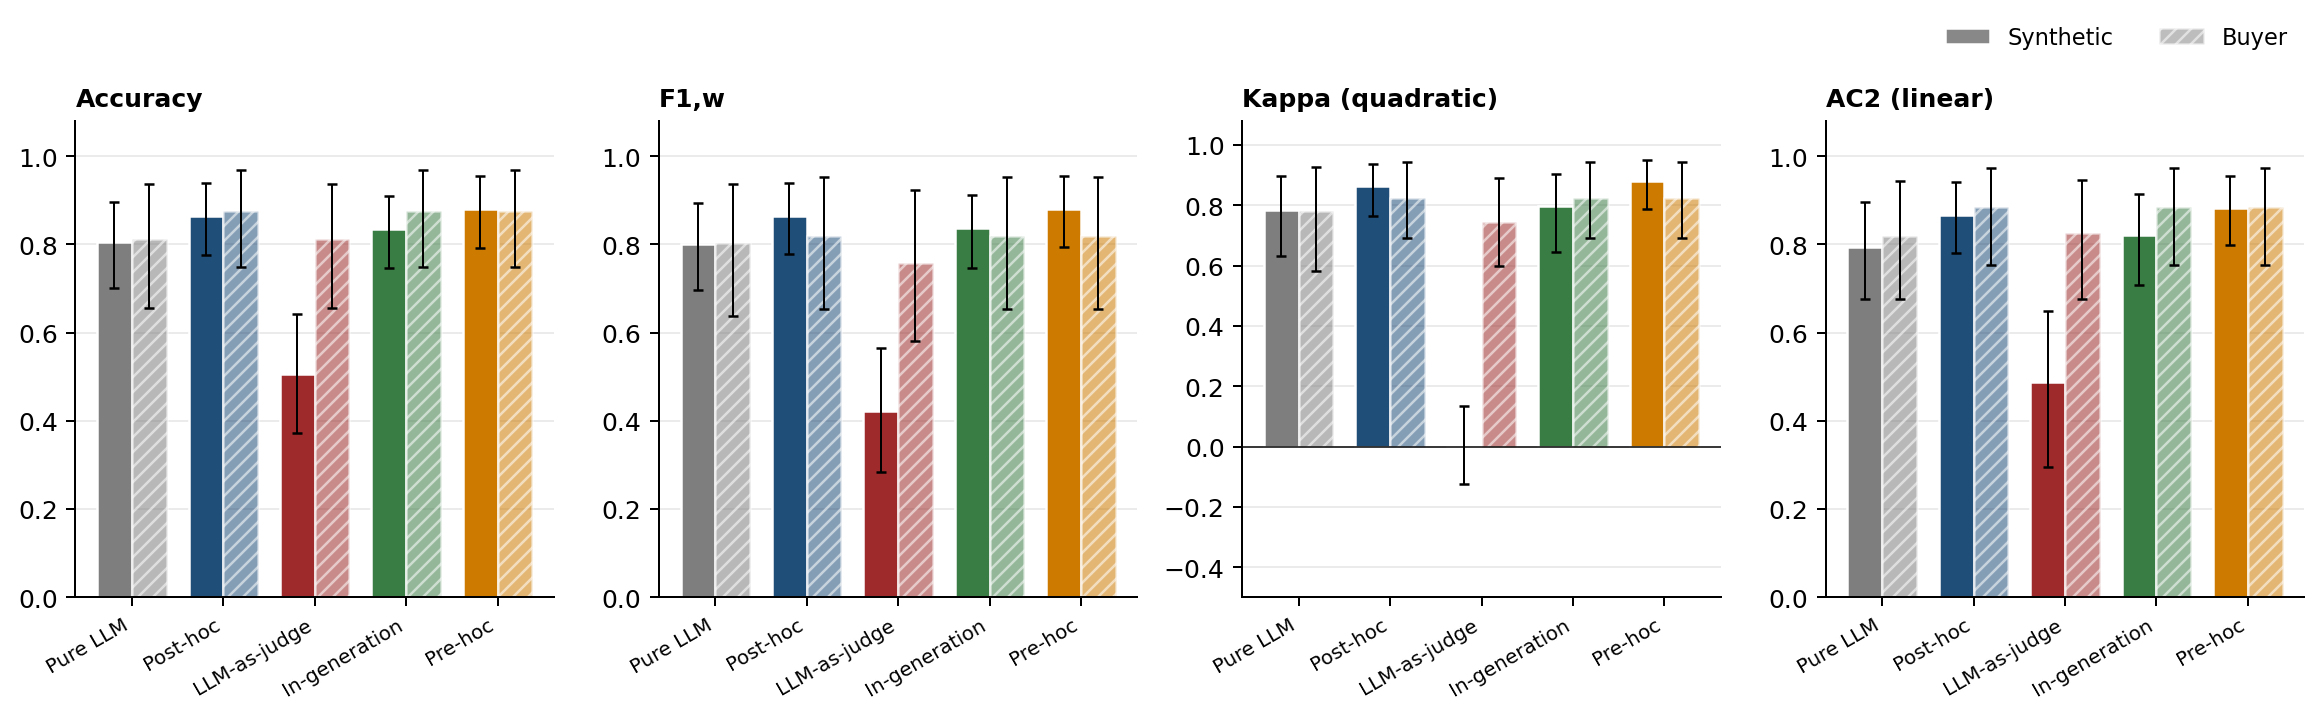
\includegraphics[width=0.85\textwidth]{Figures/fig_5_metrics_grid.png}
\caption{Disposition metrics by design: synthetic (solid) and buyer (hatched), with 95 per cent bootstrap intervals.}
\label{fig:results:metrics}
\end{figure}

\begin{figure}[htb]
\centering
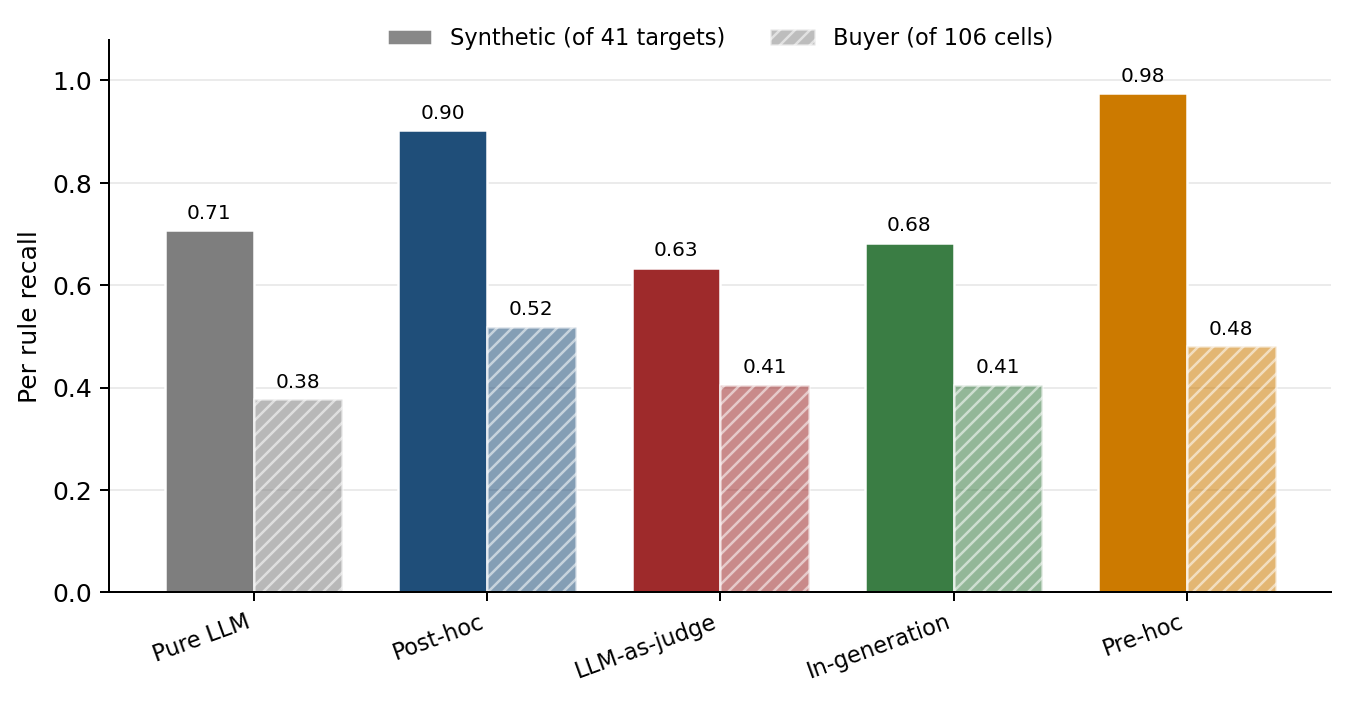
\includegraphics[width=0.8\textwidth]{Figures/fig_5_recall_bars.png}
\caption{Per rule recall by design on the synthetic sample (over the 41 evaluable single rule mutant targets) and the buyer sample (over 106 rule cells). R11 and R18 are excluded (Section~\ref{sec:results:regimes}).}
\label{fig:results:recallbars}
\end{figure}

On the synthetic sample, 3 things stand out. First, 4 of the 5 designs score between 0.81 and 0.88 on accuracy, but the LLM-as-judge design collapses to 0.51, with a weighted kappa of $-0.01$ (chance level). It is consistently too harsh: 28 of its 33 errors are over-rejections, and it fails all 9 clean single rule PASS controls, where every other design passes 6 or 7. Second, the 2 designs that route every deterministic rule through the enforcer lead on rule recall, pre hoc at 40 of 41 and post hoc at 37 of 41, against 26 to 29 for the rest. Third, accuracy and rule recall do not track each other, because a disposition turns only on the most severe firing while recall needs every target firing caught; this is why the in generation design reaches 0.84 accuracy but only 0.68 recall.

On the buyer sample the designs fall into 2 bands. The 3 enforcer bearing designs all reach 0.88 accuracy and are identical on the other 3 metrics; the 2 enforcer free designs reach 0.81. So the metrics separate enforcer from no-enforcer, but they do not separate the 3 enforcer positions. Those 3 differ only on rule recall: post hoc catches 55 of the 106 rule cells, pre hoc 51 and in generation 43. Post hoc leads here because its override recovers missed firings while keeping the model's own answers on the language model rules.


\subsection{Multi-rule interaction scenarios}
\label{sec:results:multirule}

The 17 multi-rule scenarios (SYN-M01 to SYN-M17) place 2 or 3 defects on the same ASN at once, to test whether each design still reaches the correct disposition when violations interact. Table~\ref{tab:synthetic_multirule} reports the outcome. The designs are close: the pure LLM design gets 16 of 17 right and the 3 enforcer bearing designs 15 each. Two scenarios account for the misses. SYN-M13, an intended clean PASS control, is routed to REVIEW by every design because the generated fixture carries inadvertent triggers, an early delivery placed before a fixed notice date and a within tolerance quantity that the line total check still flags, so it tests the fixture rather than the designs. SYN-M10 is missed only by the 3 enforcer designs: its partial shipment is routed to REVIEW where the construction expects REJECT, the same partial-shipment grading tension dissected for case P-48 (Section~\ref{sec:results:p48}). The LLM-as-judge design is again weakest at 13 of 17. Rule coverage, the share of the 38 stacked defects (2 or 3 per scenario across the 17 scenarios) each design flags, matters less, since the disposition turns on the single most severe firing; here the post hoc and pre hoc designs catch 34 of 38, against 27 for the LLM-as-judge design. The gaps are small, 1 to 3 scenarios, but the direction matches the single rule block: the LLM-as-judge design again loses the most dispositions.

\begin{table}[htb]
\centering
\caption{Multi-rule scenarios (SYN-M01--M17): correct dispositions and stacked-firing coverage per design. R18 tracker artefacts are excluded from coverage.}
\label{tab:synthetic_multirule}
\footnotesize
\begin{tabular}{@{}lccl@{}}
\toprule
\textbf{Design} & \textbf{Disposition match} & \textbf{Rule coverage} & \textbf{Scenarios missed} \\
\midrule
pure LLM      & 16/17 & 31/38 & SYN-M13 \\
post hoc      & 15/17 & 34/38 & SYN-M10, SYN-M13 \\
LLM-as-judge  & 13/17 & 27/38 & SYN-M02, SYN-M04, SYN-M12, SYN-M13 \\
in generation & 15/17 & 28/38 & SYN-M10, SYN-M13 \\
pre hoc       & 15/17 & 34/38 & SYN-M10, SYN-M13 \\
\bottomrule
\end{tabular}
\end{table}


\subsection{Paired contrasts between designs}
\label{sec:results:significance}

The paired contrasts take the pre hoc design as the reference. The McNemar test is symmetric, so the p-value and Cohen's h of a pair do not depend on which design is named the reference; the choice only fixes which 4 contrasts form the Holm-corrected family. Pre hoc is the natural anchor because it is the design this study recommends, the one that matches the others on disposition agreement while leading on cost, latency and reproducibility (Section~\ref{sec:results:position}), so each contrast asks the decision relevant question: does any alternative differ from the design that would be deployed? The 4 contrasts map onto the research questions: against the pure LLM baseline and the LLM-as-judge auditor for RQ.1, and against the post hoc and in generation realisations for RQ.2.

The full paired contrast table, with discordant counts, McNemar p-values and Cohen's h for every pair on both samples, is in Appendix~\ref{app:dispmetrics} (Table~\ref{tab:results:significance}).

One contrast survives correction: on the synthetic sample the pre hoc design beats the LLM-as-judge design on 27 discordant cases to 2, with an exact McNemar p below 0.001 after Holm and a large effect size of h equal to 0.85. Every other contrast is negligible to small and none other survives correction; against the post hoc and in generation realisations the discordant counts are tiny (2/1 and 4/1 on synthetic, 0/0 on buyer), so the 3 enforcer positions are indistinguishable. The single reliable separation is therefore the collapse of the LLM auditor, not a ranking among the enforcer positions. Figure~\ref{fig:results:forest} shows this: only the synthetic LLM-as-judge contrast clears the large effect band.

As a check, the same comparisons were run again on all 100 cases together. The judge design still fails clearly, and the 3 enforcer positions are still too close to separate, so combining the buyer and synthetic samples tells the same story. The main accuracy comparisons are not combined this way, because the number of synthetic cases was a design choice, and adding them in would make the result look stronger than the real case evidence supports.

\begin{figure}[htb]
\centering
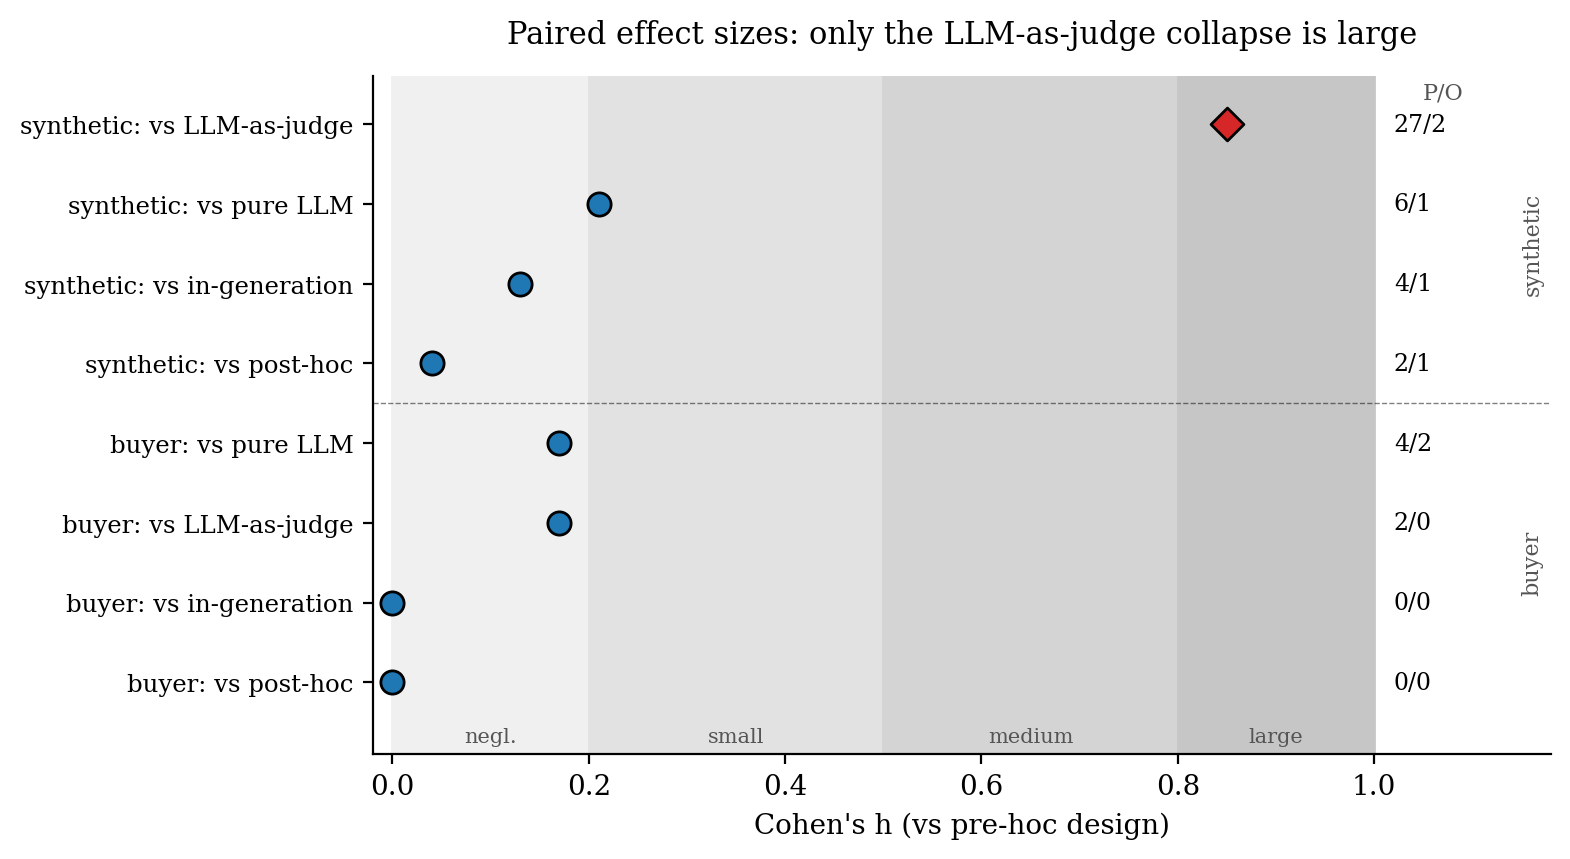
\includegraphics[width=0.86\textwidth]{Figures/fig_5_forest.png}
\caption{Paired effect sizes (Cohen's h) against the pre hoc reference. Only the synthetic LLM-as-judge contrast is large and Holm-significant.}
\label{fig:results:forest}
\end{figure}


\subsection{Per rule behaviour, rule regimes and severity-weighted F1}
\label{sec:results:regimes}

Per rule behaviour spans 2 rule populations: the 8 deterministic regime rules, whose verdict the enforcer can override, and the 14 language model regime rules, whose verdict only the model produces. In the pure LLM and LLM-as-judge designs the deterministic regime rules are left to the model, so their figures show how the model alone does on the rules the others enforce.

This is where the enforcer's advantage lies. Across the 20 evaluable rules, post hoc and pre hoc catch all 20, pure LLM 16, and in generation and LLM-as-judge 14 each. The misses concentrate on a few computation heavy rules that need a recomputed severity, a cumulative quantity or a careful field read: R06 (line item completeness), R17 (multi-PO consolidation), R20 (weight plausibility), R21 (mandatory packaging fields) and R22 (cumulative order fulfilment). Of these only R06 sits in the deterministic regime, where the enforcer recomputes it directly; the others remain in the language model regime, so the enforcer bearing designs recover them through the model rather than by deterministic recomputation, most cleanly under pre hoc, where scoping the model to fewer rules lifts its performance on them. Its value is therefore concentrated on a handful of rules the model handles unreliably under full instruction density, not on the register as a whole.

The 2 rules outside the recall count behave as expected: R11 (schema compliance) is an entry check that yields no rule level verdict, and R18 (duplicate submission) is caught by the separate re-submission check of Section~\ref{sec:method:enforcer:realisations}, where the 3 designs carrying the deterministic tracker flag the engineered duplicate and the pure LLM design does not. The severity weighted macro F1 by rule regime is in Appendix~\ref{app:dispmetrics} (Table~\ref{tab:results:fwslices}); it runs lower than the disposition accuracies because it averages over every rule, including rarely firing ones, and its ordering matches the recall table.


\subsection{Cost and latency}
\label{sec:results:cost}

Cost and latency are observed on the 28 production cases, the recurring operating stream; the 4 pre-integration cases are one-off integration events, excluded here but kept in the 32 case disposition results, and the synthetic cases do not represent live cost. The full operational spread is in Appendix~\ref{app:operational}, together with the latency distribution (Figure~\ref{fig:results:latency}) and the cost/accuracy trade-off (Figure~\ref{fig:results:pareto}).

The pre hoc design is the cheapest and fastest by a clear margin, at EUR 0.073 per ASN and a median latency of 7.89 seconds, and its distribution is the tightest, with a latency standard deviation of 1.73 seconds against 5.70 or more for every other design. The in generation design is the most expensive, at EUR 0.171 per ASN, a cost ratio of 2.34 against the pre hoc design. The reason is prompt size: the pre hoc design fixes the deterministic verdicts before the model call and asks the model to reason over the language model rules only (prompt mean 9,870 tokens), while the in generation design carries tool definitions in the prompt and interleaves tool calls in the response (prompt mean 26,244 tokens).

At this throughput the absolute compute cost is small, and the operationally significant saving is the analyst time the pipeline removes, the same for every design because they share the disposition output. Chapter~\ref{chap:conclusions} works that saving through and weighs it against the compute cost.


\subsection{Supplier context ablation}
\label{sec:results:rag}

This subsection answers RQ.3, whether conditioning the prompt on a supplier's historical failure record improves disposition accuracy. The supplier conditioned prompting layer injects a retrieved supplier history line into the prompt; the method, including the leave-one-out and placebo protocol, is defined in Section~\ref{sec:method:supplier}. Its effect is isolated by an ablation on the 18 production cases swept under all arms: retrieval off, retrieval on under a leave-one-out protocol, and a wrong supplier placebo. Table~\ref{tab:rag_ablation} reports disposition accuracy and the language model regime F1, the only rules the prior can move. The placebo arm is run only for the enforcer free designs (pure LLM and LLM-as-judge): it isolates whether the model is swayed by an authoritative-looking but wrong history, a property of the model that the enforcer would override anyway, so n/a marks the arm as not run rather than missing for the enforcer bearing designs.

\begin{table}[htb]
\centering
\caption{Supplier context ablation on 18 production cases: disposition accuracy and language model-regime F1 across retrieval off, on (leave-one-out) and placebo.}
\label{tab:rag_ablation}
\footnotesize
\begin{adjustbox}{max width=\textwidth}
\begin{tabular}{@{}lcccccc@{}}
\toprule
& \multicolumn{3}{c}{\textbf{Accuracy}} & \multicolumn{3}{c}{\textbf{LM-regime F1}} \\
\cmidrule(lr){2-4} \cmidrule(lr){5-7}
\textbf{Design} & \textbf{Off} & \textbf{On} & \textbf{Placebo} & \textbf{Off} & \textbf{On} & \textbf{Placebo} \\
\midrule
pure LLM      & 0.778 & 0.778 & 0.778 & 0.365 & 0.352 & 0.357 \\
post hoc      & 0.778 & 0.778 & n/a   & 0.454 & 0.337 & n/a   \\
LLM-as-judge  & 0.667 & 0.667 & 0.611 & 0.332 & 0.337 & 0.344 \\
in generation & 0.667 & 0.778 & n/a   & 0.483 & 0.382 & n/a   \\
pre hoc       & 0.778 & 0.778 & n/a   & 0.358 & 0.278 & n/a   \\
\bottomrule
\end{tabular}
\end{adjustbox}
\end{table}

The measured finding is a null effect, so the answer to RQ.3 is negative on this sample. Accuracy does not move between arms on 4 of the 5 designs, and across all 5 at most 2 of the 18 dispositions change. The prior is read rather than ignored, since it shifts the language model regime F1, but no disposition follows, so the verdict is robust to it.

A strict past-only variant conditions each case only on the supplier's earlier cases, leaving the first case of each supplier cold, so 11 of the 18 cases carry a non-empty prior. This variant reproduces the null. Accuracy stays at the no-context baseline on 4 of the 5 designs and moves by a single case on the other 2, a net of zero flips against the off arm. Removing the look-ahead therefore reveals no hidden benefit, and closes the objection that the leave-one-out result masked a real effect by drawing on future cases. On this sample reliability comes from the deterministic enforcer, not the retrieved supplier context, whether that context is read across all of a supplier's cases or only its past. This is taken up in Chapter~\ref{chap:conclusions}.


\subsection{Cross-model robustness}
\label{sec:results:crossmodel}

The results above use a single language model (Section~\ref{sec:method:constraints}). To test whether the separation between the designs is specific to that model, the buyer cohort was also evaluated under a second model from a different family, Mistral-Large-3 on Azure AI Foundry, holding the pipeline, the prompts and the rule logic fixed. Three provider side settings differ on the second model: the seed and schema constrained outputs are unavailable and were disabled, R18 was excluded from the sweep, and the in generation design needed a transport accommodation to invoke its tools; the deterministic checks themselves are identical. Table~\ref{tab:results:crossmodel} reports disposition accuracy per design on the 32 buyer cases for both models, and Figure~\ref{fig:results:crossmodel} plots the same values as a dot plot.

\begin{table}[htb]
\centering
\caption{Cross-model robustness: disposition accuracy on the 32 buyer cases per design, under the primary model (gpt-5.4-mini) and a second model from a different family (Mistral-Large-3).}
\label{tab:results:crossmodel}
\footnotesize
\begin{tabular}{@{}lcc@{}}
\toprule
\textbf{Design} & gpt-5.4-mini & Mistral-Large-3 \\
\midrule
pure LLM      & 0.81 & 0.69 \\
post hoc      & 0.88 & 0.84 \\
LLM-as-judge  & 0.81 & 0.72 \\
in generation & 0.88 & 0.81 \\
pre hoc       & 0.88 & 0.81 \\
\bottomrule
\end{tabular}
\end{table}

\begin{figure}[htb]
\centering
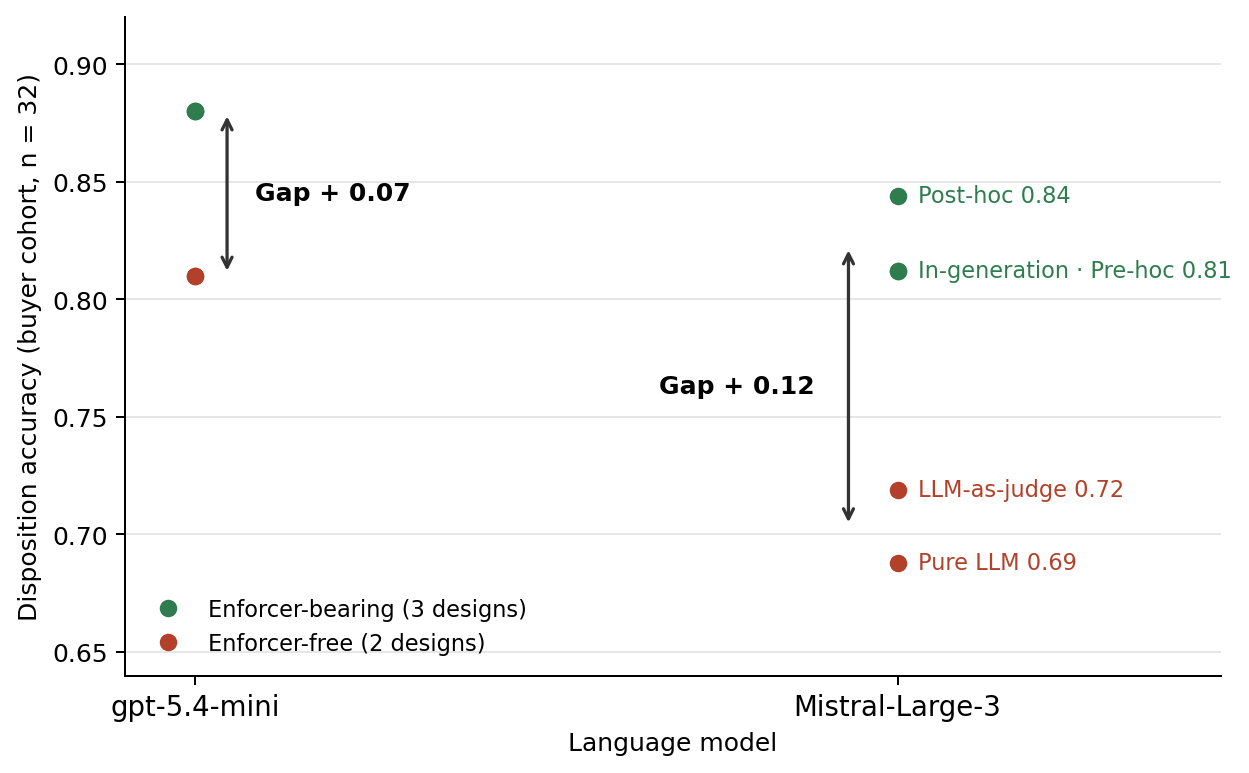
\includegraphics[width=0.82\textwidth]{Figures/fig_5_crossmodel_slopegraph_2.png}
\caption{Cross-model enforcer gap: buyer cohort disposition accuracy of the 5 designs under the primary model (gpt-5.4-mini) and a second model from a different family (Mistral-Large-3).}
\label{fig:results:crossmodel}
\end{figure}

Under Mistral-Large-3 the absolute accuracies are lower, as expected for a model less suited to the task, but the enforcer versus no enforcer separation reproduces and in fact widens. The 3 enforcer bearing designs average 0.82 against 0.70 for the 2 enforcer free designs, a gap of 0.12, against 0.07 on the primary model. The separation is therefore not an artefact of the primary model. The gap widens for a simple reason: the enforcer recomputes the deterministic rules identically regardless of the model, so on a weaker model the enforcer free designs lose more accuracy while the enforcer bearing designs are protected. Practically, this de-risks model choice: a weaker or cheaper model can be deployed behind the enforcer with bounded loss, because the computable rules are protected. The safety asymmetry also replicates only where the enforcer's authority is hard: under the second model the post hoc and pre hoc designs still never under-reject, while the in generation design lets 2 defective ASNs through, so the soft realisation is the first to lose the safety property as the model weakens. The second model also ran several times slower per case on the same pipeline, so the primary model keeps the operational edge. The reported values are the majority of 3 replays per case. Appendix~\ref{app:crossmodel} gives the per-design confusion matrices, the error direction, the reproducibility across replays and the per-run latency on the second model.


%% =================================================================
\section{Position of the deterministic enforcer}
\label{sec:results:position}

The 3 enforcer positions, post hoc, in generation and pre hoc, do not separate on disposition agreement (Section~\ref{sec:results:comparison}): they are identical on the buyer sample and within run-to-run noise on the synthetic one (Table~\ref{tab:results:significance}). The decision between them therefore rests on the operational criteria of RQ.2: cost, latency and reproducibility, and on all 3 the pre hoc design leads. It is the cheapest and the fastest, with the per-design figures in Section~\ref{sec:results:cost}, and the most reproducible, Table~\ref{tab:results:repro} reporting how often each design returns an identical verdict across the 5 runs. Figure~\ref{fig:results:rq2} summarises the answer: the 3 positions overlap on accuracy and separate only on the operational axes, where the pre hoc design leads each one.

\begin{figure}[htb]
\centering
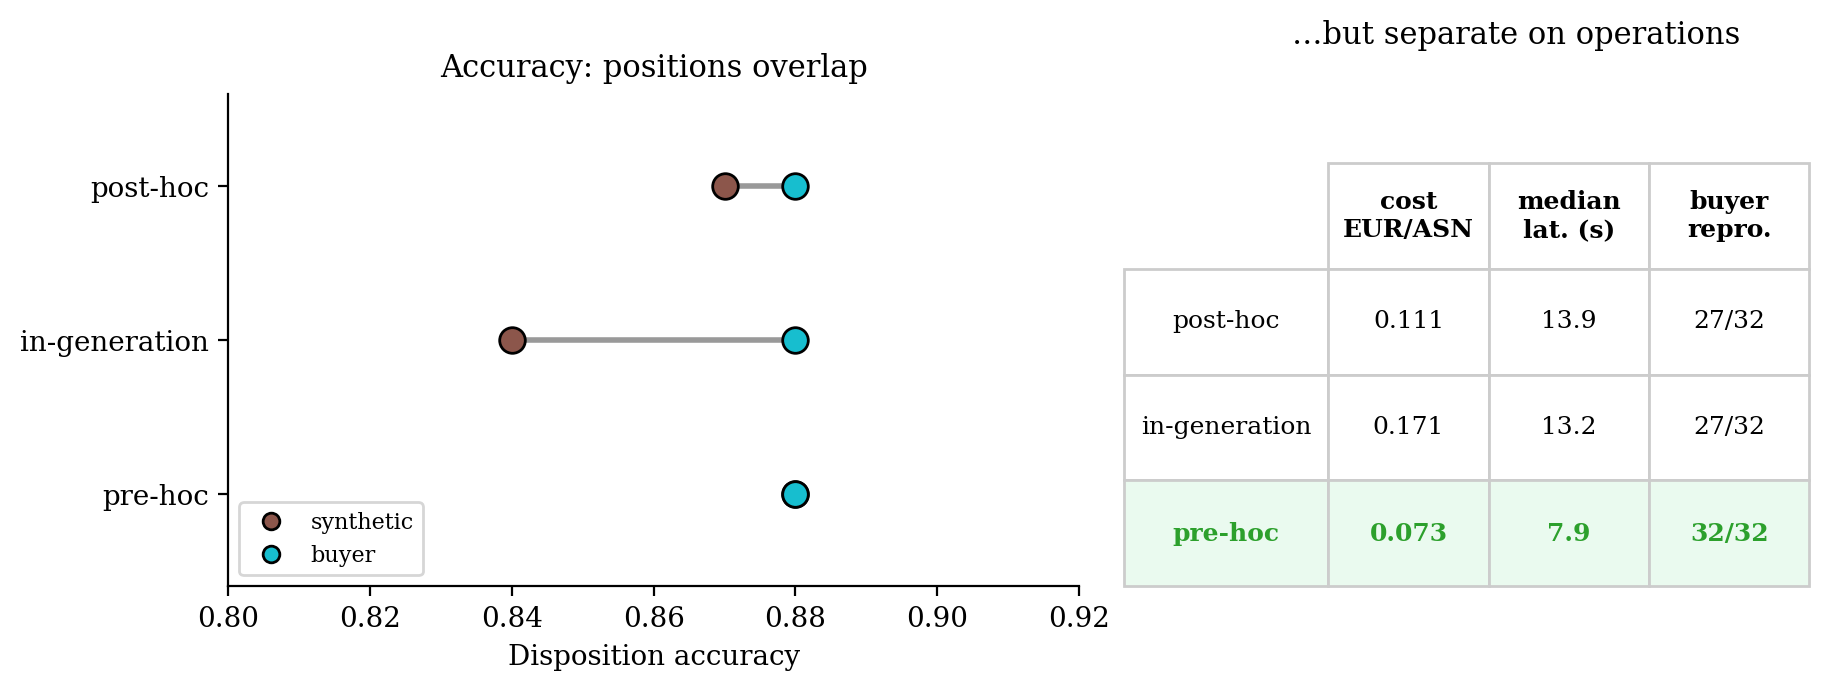
\includegraphics[width=0.85\textwidth]{Figures/fig_5_rq2_dumbbell.png}
\caption{The 3 enforcer positions: identical on accuracy (left), separated only on cost, latency and reproducibility (right), where the pre hoc design leads.}
\label{fig:results:rq2}
\end{figure}

Verdict reproducibility across the 5 runs is reported in Appendix~\ref{app:dispmetrics} (Table~\ref{tab:results:repro}). On the buyer sample the pre hoc design is the only enforcer position whose disposition is identical in all 5 runs, 32 of 32, with a per-run accuracy standard deviation of 0.000. The post hoc and in generation designs each repeat 27 of 32 buyer verdicts, and the post hoc per-run accuracy ranges from 0.81 to 0.94. On the synthetic sample the pre hoc design is again the most stable, at 66 of 67, against 61 of 67 for the post hoc design and 43 of 67 for the LLM-as-judge design, and is therefore the recommended position. The post hoc design retains the per rule recall edge on the buyer sample, 0.52 against 0.48, which matters where the per rule audit trail is the product; this does not change the disposition tie. The in generation design matches the others on agreement but is the most expensive and holds no compensating advantage.

\subsection{What the enforcer does at each position}
\label{sec:results:actions}

The action audit explains why the 3 positions tie on agreement while differing operationally. The post hoc enforcer works downstream, correcting the model after the fact with 32 verdict overrides and 43 missing-firing injections; Table~\ref{tab:results:flow} shows what those corrections achieve against the pure LLM design that shares its model call, lifting the correct count and cutting over-rejections on both cohorts. The in generation design consults the deterministic tools during generation, so overrides are unnecessary and the only residual action is severity capping. The pre hoc design records 0 actions of any kind: by fixing the deterministic verdicts before the model call it prevents the error upstream rather than correcting it downstream, which is also why it leads on cost, latency and reproducibility. The per-design action counts and the severity-capping counterfactual are in Appendix~\ref{app:dispmetrics} (Tables~\ref{tab:results:actions} and~\ref{tab:results:capping}).

\begin{table}[htb]
\centering
\caption{What the post hoc enforcer corrects, against the pure LLM design that shares its model call.}
\label{tab:results:flow}
\footnotesize
\begin{tabular}{@{}lcccccc@{}}
\toprule
& \multicolumn{3}{c}{\textbf{Synthetic (67)}} & \multicolumn{3}{c}{\textbf{Buyer (32)}} \\
\cmidrule(lr){2-4} \cmidrule(lr){5-7}
\textbf{Outcome} & \textbf{pure LLM} & \textbf{post hoc} & \textbf{Change} & \textbf{pure LLM} & \textbf{post hoc} & \textbf{Change} \\
\midrule
Correct dispositions & 54 & 58 & $+4$ & 26 & 28 & $+2$ \\
Over-rejections      & 8  & 5  & $-3$ & 6  & 4  & $-2$ \\
Under-rejections     & 5  & 4  & $-1$ & 0  & 0  & 0    \\
\bottomrule
\end{tabular}
\end{table}

These auxiliary operations are the enforcer's output contract rather than per-design features: whichever realisation runs, injection guarantees no owned rule is missing and capping guarantees its severity matches the register, so they are kept as safety nets against language model non-determinism even where this corpus triggered them 0 times. Where capping changes a disposition it always moves it toward the ground truth. The firing pattern is itself the finding: post hoc corrects after the fact, in generation needs only capping, and pre hoc needs nothing.


%% =================================================================
\section{Error analysis}
\label{sec:results:errors}

\subsection{Error direction}
\label{sec:results:direction}

Disposition errors fall into 2 kinds on the ordered scale PASS, REVIEW, REJECT. An over-rejection is a verdict more severe than the analysts', and an under-rejection is a verdict less severe. The two carry different operational weight: an over-rejection sends a sound ASN to manual review, while an under-rejection lets a defective ASN through. The under-rejection is the unsafe error, because it is the one that reaches the buyer.

On the buyer sample, every error that any design makes is an over-rejection: of the verdicts that differ from the consensus, all are more severe than it and none less severe, as the buyer panel (top row) of Figure~\ref{fig:results:confusion} shows, where every off-diagonal cell sits above the diagonal and none below. The errors split into 2 mechanisms. The first is severity escalation: of the 15 cases the panel marked REVIEW, the pure LLM design pushes 4 to REJECT and the LLM-as-judge design 2, while the 3 enforcer bearing designs push none, because the enforcer recomputes each deterministic rule's registered severity instead of trusting the model's. The second is completeness over-review: of the 4 PASS cases, every design escalates 2 to 4 to REVIEW on packaging completeness grounds (R21, which asks whether the mandatory packaging fields are present), which the enforcer does not suppress, because the question is which rule fires, not how severe. On the synthetic sample, where the mutants engineer genuine defects, under-rejections do occur, 3 to 6 per design, visible below the diagonal in the synthetic panel (bottom row) of Figure~\ref{fig:results:confusion}; the LLM-as-judge design also adds 28 over-rejections, the harshness that Section~\ref{sec:results:p48} dissects.

\begin{figure}[htb]
\centering
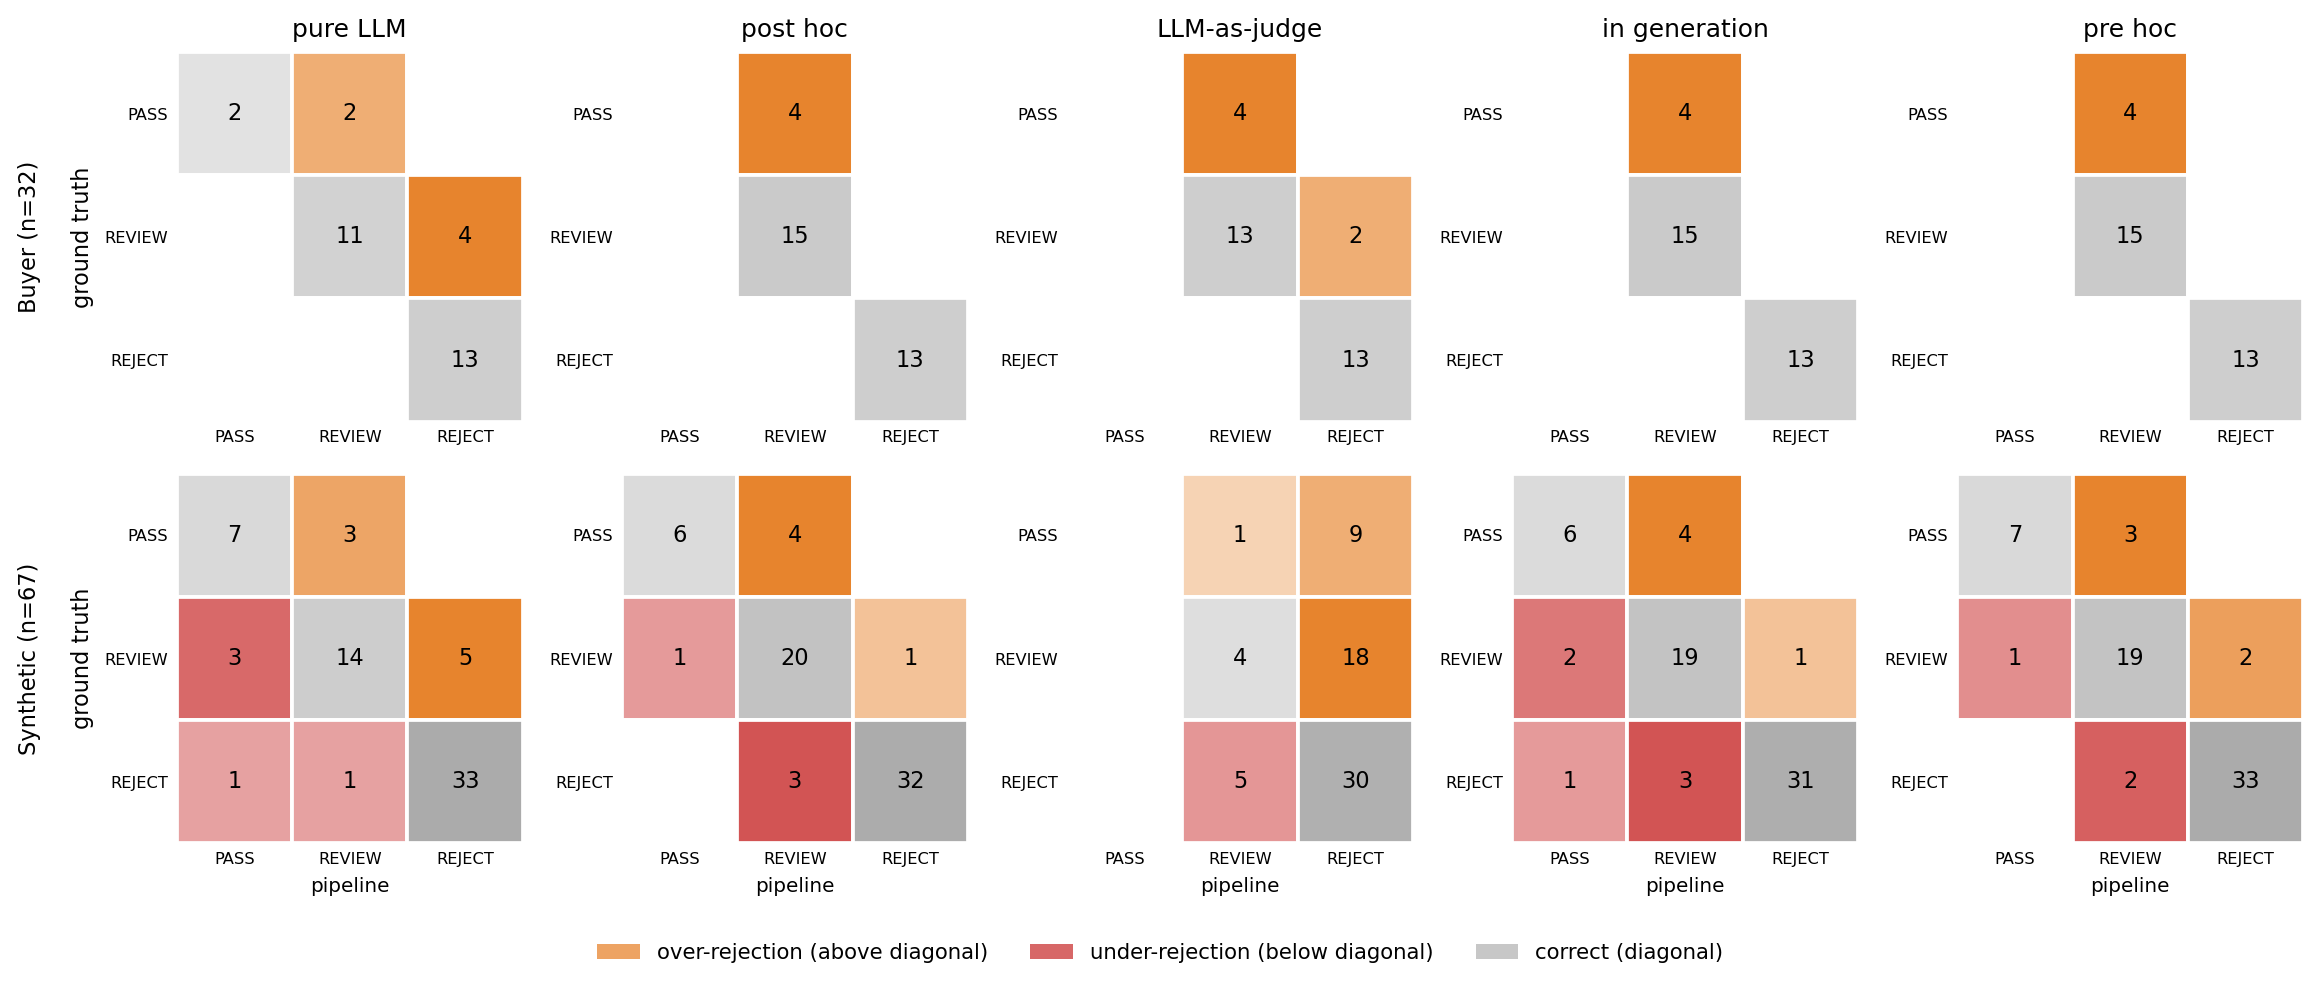
\includegraphics[width=\textwidth]{Figures/fig_5_confusion_panels.png}
\caption{Per-design disposition confusion matrices, buyer cohort (top, n=32) and synthetic cohort (bottom, n=67). Rows are the consensus, columns the pipeline; above the diagonal is over-rejection, below is under-rejection.}
\label{fig:results:confusion}
\end{figure}

Reading the figure, the safety asymmetry is what matters. Over-rejection, the mass above the diagonal, is the tolerable error: a sound ASN is sent to a reviewer, which costs time but never lets a defect through. Under-rejection, below the diagonal, is the unsafe error, because the defect reaches the buyer. No design under-rejects on the buyer cohort, so all 5 are safe in this sense and differ only in how much, and how harshly, they over-review. The 3 enforcer bearing designs keep their only error in the mildest cell, escalating PASS cases to REVIEW on completeness grounds, and never push a genuine REVIEW to REJECT, because the enforcer holds the deterministic severities. The 2 enforcer free designs are harsher: they also bounce genuine REVIEW cases to REJECT, 4 for the pure LLM design and 2 for the LLM-as-judge design, which returns a workable shipment to the supplier and is the costlier over-rejection the enforcer removes.


\subsection{Error walkthrough: cases P-48 and SYN-M10}
\label{sec:results:p48}

Case P-48 is a representative example of the over-rejection pattern, because its rule signature, a multiple purchase order shipment under partial delivery, recurs across the REJECT subset of the buyer sample. It is a shipment from an Austrian supplier covering 4 purchase orders, each only partially delivered. The analysts' verdict is REVIEW, with several warning-level firings and no critical firing.

The designs diverge on the severity of rule R06 (line item completeness, which asks whether every PO line has a matching ASN item), and that severity decides the disposition. R06 fires here because the partial deliveries leave PO lines uncovered, and its deterministic check grades exactly this situation, missing lines that trace to a declared partial delivery, as warning rather than critical. The pure LLM design escalates R06 to critical and returns REJECT. The LLM-as-judge design escalates R06 to critical on all 4 purchase orders, invents a quantity violation (R01, shipped quantity match) by confusing line level and total level quantities, and asserts a duplicate shipment flag (R18) with no supporting evidence, returning REJECT. The 3 enforcer bearing designs all hold R06 at warning, because each routes it through the deterministic enforcer, and all 3 return REVIEW in agreement with the analysts.

Case P-48 exposes 3 independent failure modes of the LLM-as-judge design, each enough on its own to caution against it. It is too harsh: its severity prior runs more severe than the analysts', as the 28 synthetic over-rejections and the 9 of 9 failed single rule PASS controls show. It hallucinates: it invents rule firings with no anchor in the payload, as with R01 and R18 here. And it is unstable: it is the least reproducible design, repeating only 21 of 32 buyer verdicts and 43 of 67 synthetic verdicts. Together with the only Holm-significant contrast in the chapter, these 3 faults rule the pattern out.


The same pattern recurs on the pre-integration sample. The 4 pre-integration cases (PI-01 to PI-04) all carry a consensus REVIEW; 3 are returned REVIEW by every design, while the 4th, PI-04, a partial delivery case, splits the designs exactly as P-48 does: the pure LLM and LLM-as-judge designs escalate it to REJECT, the 3 enforcer bearing designs hold it at REVIEW. The per-case audit is in Appendix~\ref{app:dispmetrics} (Table~\ref{tab:results:pi}).

The same calibration produces the opposite error on the synthetic sample. Scenario SYN-M10 combines a partial shipment with missing packaging fields, and its disposition by construction is REJECT. The 3 enforcer bearing designs return REVIEW, grading the partial shipment as tolerable, while the 2 enforcer free designs reject it. The deterministic severity that grades partial deliveries as warning, and so prevents the over-rejection on P-48, here leaves the case at REVIEW where the construction expects REJECT, and yields an under-rejection. The divergence is confined to this engineered case and does not occur on the buyer cohort, so it marks the boundary of the enforcer's partial-shipment policy rather than a failure on the real sample.



%% =================================================================
\section{Chapter conclusion}
\label{sec:results:conclusion}

This chapter compared the 5 designs on the synthetic and buyer samples. The deterministic enforcer is the component that separates them: the 3 enforcer bearing designs lead on disposition accuracy and rule recall, and the LLM-as-judge design, the only statistically reliable contrast, is ruled out on harshness, hallucination and instability. The 3 enforcer positions tie on disposition agreement, so the choice between them is operational, and the pre hoc design leads on cost, latency and reproducibility. The supplier history prior has no measurable effect, and a second model from a different family reproduces and widens the enforcer gap, confirming the separation is a property of the architecture rather than the model. Chapter~\ref{chap:conclusions} answers the research questions against these findings and sets out the limitations.
